%%% Please replace what is within each curly bracket with the correct information below. %%%
%%% The first field is already filled in for you.  %%%
\def\ClassName {CS188} % Your course 
\def\NameLast {Chen}  % Your last name
\def\NameFirst {Jianzhong}  % Your first name
\def\SID{23478230}  % Your SID
\def\Email{chenjianzhong@berkeley.edu} % Your pandagrader email
\def\Collaborators{None} % Any collaborators

\def\OneA{

\item \mcqb $A$ \item \mcqb $B$ \item \mcqs $C$ \item \mcqb $D$ \item \mcqb $E$ \item \mcqb $F$

}

\def\OneB{
\begin{itemize}[label=, itemsep=12pt, topsep=12pt]

\item \mcqb $-\infty$ \item \mcqb $1/2$ \item \mcqb $-2$ \item \mcqb $1$ \item \mcqb $-1$
\item \mcqb $2$ \item \mcqb $-1/2$ \item \mcqb $\infty$ \item \mcqs $0$
\end{itemize}
\end{multicols}

\begin{multicols}{2}
\begin{itemize}[label=, itemsep=12pt, topsep=12pt]
\item \mcqb $Can$ be determined but is not equal to any of the provided options
\item \mcqb $Cannot$ be determined from the information provided
\end{itemize}
}

\def\OneC{

\item \mcqs LL-Train would remain the same.
\item \mcqb LL-Train would go up.
\item \mcqb LL-Train would go down.
\item \mcqs LL-Test would remain the same.
\item \mcqb LL-Test would go up.
\item \mcqb LL-Test would go down.
}
\def\OneCExplanation{
Since LL-Train and LL-Test are under the limit of infinite data, and Laplace smoothing will only add only a small amount of samples, which is too few to change the value of LL-Train and LL-Test.
}

\def\OneD{

\begin{tabular}{llll}
Small amount of training data: &
\mcqb $A \qquad$ & \mcqs $B \qquad$ & \mcqb $C \qquad$ \\  \\ \\
Medium amount of training data: &
\mcqs $A$ & \mcqb $B$ & \mcqb$C$ \\ \\ \\
Large amount of training data: &
\mcqb $A$ & \mcqb $B$ & \mcqs$C$ \\ \\ \\
\end{tabular}
}

\def\OneDExplanation{
With fewer data, a simple Bayes' net can generalize pretty well, but a complex Bayes' net will overfit. However, for a large amount of data, a simple Bayes' net will underfit, but a complex Bayes' net can simulate the actually distribution.
}

\def\TwoA{
$p(A=+m|B=
+m,C=+m)=\frac{p(A=+m,B=
+m,C=+m)}{\sum_a{p(A=a,B=+m,C=+m)}}=\frac{p(A=+m)p(X=+m|\pi(X)=+m)p(X=+m|\pi(X)=+m)}{\sum_a{p(A=a)p(X=+m|\pi(X)=a)p(X=+m|\pi(X)=a)}}=\frac{0.5*0.9*0.9}{0.5*0.9*0.9+0.5*0.1*0.1}=\frac{81}{82}$
}

\def\TwoB{
$p(D=+m|A=+m)=\frac{0.9^2+0.1^2}{0.9^2*0.1^2+2*0.9*0.1}=\frac{41}{50}$
}

\def\TwoC{
$EU=p(D=+m|A=+m)*(-1)+(1-p(D=+m|A=+m))*1=-0.64$
}

\def\TwoD{
$VPI=1-0.64=0.36$
}

\def\TwoE{
Since D is independent from F given A, so the VPI of F given D=+m is 0.
}

\def\TwoF{
\begin{center}
\begin{tabular}{lllll}
\mcqs $A \phantom{----}$  & \mcqs $B \phantom{----}$  & \mcqb $C \phantom{----}$  & \mcqb $E \phantom{----}$   \\ [1em]
\mcqb $F \phantom{----}$  & \mcqb $G \phantom{----}$  & \mcqb $H \phantom{----}$  & \mcqb $I \phantom{----}$  & \mcqb $J \phantom{----}$   \\ [1em]
\mcqb $K \phantom{----}$  & \mcqb $L \phantom{----}$  & \mcqb $M \phantom{----}$  & \mcqb $N \phantom{----}$  & \mcqb $O \phantom{----}$   \\ [1em]
\end{tabular}
\end{center}
}
\def\TwoFExplanation{
Because D is dependent on B, and B is dependent on A.
}

\def\TwoG{
\begin{center}
\begin{tabular}{lllll}
\mcqs $A \phantom{----}$  & \mcqs $B \phantom{----}$  & \mcqb $C \phantom{----}$  & \mcqb $E \phantom{----}$   \\ [1em]
\mcqb $F \phantom{----}$  & \mcqb $G \phantom{----}$  & \mcqb $H \phantom{----}$  & \mcqb $I \phantom{----}$  & \mcqb $J \phantom{----}$   \\ [1em]
\mcqb $K \phantom{----}$  & \mcqb $L \phantom{----}$  & \mcqb $M \phantom{----}$  & \mcqb $N \phantom{----}$  & \mcqb $O \phantom{----}$   \\ [1em]
\end{tabular}
\end{center}
}

\def\TwoGExplanation{
Same reason as F
}
%%%%%%%%%%%%%%%%%%%%%% DO NOT CHANGE ANYTHING BELOW THIS LINE %%%%%%%%%%%%%%%%%%%%%%%%%
\def \showSolutions {} 
\documentclass[twoside]{article}

\usepackage{class}
%\usepackage{verbatim}
\usepackage{fancyhdr}
\usepackage{booktabs}
\usepackage{setspace}
\usepackage{amsmath,mathrsfs}
\usepackage{multicol}
\usepackage{multirow}
\usepackage{amssymb}
\usepackage{tikz}
\usetikzlibrary{matrix}
\usepackage{graphicx}
\usepackage{subfig}
\usepackage{array}
\usepackage{xcolor}
\usepackage{float}
\usepackage{enumitem}
\usepackage{mathcomp}
\usepackage{tabularx}
\usepackage{wasysym}
\usepackage{pbox}
\usetikzlibrary{bayesnet}

% Bubbles for multiple choice questions
\newcommand{\mcqbubble}{\bigcirc}
\newcommand{\mcqbubblefill}{\Large\newmoon}

% shorthand
\newcommand{\mcqb}{$\bigcirc$\ \ }
\newcommand{\mcqs}{\solution{\mcqb}{$\Large\newmoon$\ \ }}

% pruning
\newcommand{\prune}{
\includegraphics[width=0.2in]{figures/red_x}}
% title is Written HW9
\title{Written HW9}
\begin{document}
\thispagestyle{empty}
\maketitle


\smallskip
\smallskip
\textbf{INSTRUCTIONS}

\begin{itemize}
\item \textbf{Due:} Monday, April 14th 2014 11:59 PM
\item \textbf{Policy:} Can be solved in groups (acknowledge collaborators) but must
be written up individually. However,
we strongly encourage you to first work alone for about 30 minutes total in order to simulate an exam environment.  Late homework
will not be accepted.
\item \textbf{Format:}
You must solve the questions on this handout (either through a pdf annotator, or by printing, then scanning; we recommend the latter to match exam setting). Alternatively, you can typeset a pdf on your own that has answers appearing in the same space (check edx/piazza for latex templating files and instructions).
\textbf{Make sure that your answers (typed or handwritten) are within the
dedicated regions for each question/part.  If you do not follow this format, we may deduct points.}

\item \textbf{How to submit:}  Go to www.pandagrader.com. Log in and click on the
class CS188 Spring 2014. Click
on the submission titled Written HW 9 and upload your pdf containing your answers. If this is your first time using
pandagrader, you will have to set your password before logging in the
first time.  To do so, click on "Forgot your password" on the login
page, and enter your email address on file with the registrar's office
(usually your @berkeley.edu email address). You will then receive an
email with a link to reset your password.

\end{itemize}


\begin{center}
\begin{tabular}{|r|c|}
\hline
\begin{minipage}{3cm}~\\Last Name~\\~\\\end{minipage} & \begin{minipage}[c][1cm][c]{8cm} ~ \NameLast \end{minipage}  \\
\hline
\begin{minipage}{3cm}~\\First Name~\\~\\\end{minipage} & \NameFirst \\
\hline
\begin{minipage}{3cm}~\\SID~\\~\\\end{minipage} & \SID \\
\hline
\begin{minipage}{3cm}~\\Email~\\~\\\end{minipage} & \Email \\
\hline
\begin{minipage}{3cm}~\\Collaborators~\\~\\\end{minipage} & \Collaborators \\
\hline

\end{tabular}
\end{center}



\vfill

\smallskip
\smallskip
\smallskip
\smallskip
\smallskip

\begin{center}
{\bf For staff use only}\\
\begin{Large}
\begin{tabular}{|r|r|r|}
\hline
Q. 1 & Q. 2 & Total\\
\hline

\quad/10 & \quad/20 & \qquad/30 \\
\hline
\end{tabular}\end{Large}
\end{center}


\newpage

\q{30}{CSPs}
\begin{question}[]{\bf Pacman's new house}

After years of struggling through mazes, Pacman has finally made peace with the ghosts, Blinky, Pinky, Inky, and Clyde, and invited them to live with him and Ms. Pacman. The move has forced Pacman to change the rooming assignments in his house, which has 6 rooms. He has decided to figure out the new assignments with a CSP in which the variables are Pacman \textbf{(P)}, Ms. Pacman \textbf{(M)}, Blinky \textbf{(B)}, Pinky \textbf{(K)}, Inky \textbf{(I)}, and Clyde \textbf{(C)}, the values are which room they will stay in, from 1-6, and the constraints are:
\begin{table}[h]
\centering
\begin{tabular}{ll}
i) No two agents can stay in the same room&\\
ii) \textbf{P} $>$ 3 &
vi) \textbf{B} is even\\
iii) \textbf{K} is less than \textbf{P}&
vii) \textbf{I} is not 1 or 6\\
iv) \textbf{M} is either 5 or 6&
viii) $\vert$\textbf{I}-\textbf{C}$\vert$ = 1\\
v) \textbf{P} $>$ \textbf{M}&
ix) $\vert$\textbf{P}-\textbf{B}$\vert$ = 2
\end{tabular}
\end{table}
\begin{subquestion}[1]{\bf Unary constraints}
On the grid below cross out the values from each domain that are eliminated by enforcing unary constraints.
\solution{
\begin{table}[h]
\centering
\begin{tabular}{ccccccc}
P & 1 & 2 & 3 & 4 & 5 & 6\\
B & 1 & 2 & 3 & 4 & 5 & 6\\
C & 1 & 2 & 3 & 4 & 5 & 6\\
K & 1 & 2 & 3 & 4 & 5 & 6\\
I & 1 & 2 & 3 & 4 & 5 & 6\\
M & 1 & 2 & 3 & 4 & 5 & 6\\
\end{tabular}
\end{table}
}{
\begin{table}[h]
\centering
\begin{tabular}{ccccccc}
\AnswerOneAi
\end{tabular}
\end{table}
}
\end{subquestion}
\begin{subquestion}[1]{\bf MRV}
According to the Minimum Remaining Value (MRV) heuristic, which variable should be assigned to first?\\\\
\AnswerOneAii

\end{subquestion}

\begin{subquestion}[3]{\bf Forward Checking}
For the purposes of decoupling this problem from your solution to the
previous problem, assume we choose to assign P first, and assign it the value 6. What are the resulting domains after enforcing unary constraints (from part i) and running forward checking for this assignment?
\solution{
\begin{table}[h]
\centering
\begin{tabular}{ccccccc}
P &   &   &   &  &   &  6\\
B & 1 & 2 & 3 & 4 & 5 & 6\\
C & 1 & 2 & 3 & 4 & 5 & 6\\
K & 1 & 2 & 3 & 4 & 5 & 6\\
I & 1 & 2 & 3 & 4 & 5 & 6\\
M & 1 & 2 & 3 & 4 & 5 & 6\\

\end{tabular}
\end{table}
}{
\begin{table}[h]
\begin{center}
\begin{tabular}{ccccccc}
\AnswerOneAiii
\end{tabular}
\end{center}
\end{table}

}
\end{subquestion}

\begin{subquestion}[3]{\bf Iterative Improvement}
Instead of running backtracking search, you decide to start over and run
iterative improvement with the min-conflicts heuristic for value selection. Starting with the following assignment:\\\\
P:6, B:4, C:3, K:2, I:1, M:5\\\\
First, for each variable write down how many constraints it violates in the table below.\\
Then, in the table on the right, for all variables that could be selected for assignment, put an x in any box that corresponds to a possible value that could be assigned to that variable according to min-conflicts \textbf{in the next iteration}. When marking next values a variable could take on, only mark values different from the current one.

\begin{center}
\begin{tabular}{cc}
\begin{tabular}{|c|c|}
\hline
\AnswerOneAiv
\end{tabular}
\end{tabular}
\end{center}
\end{subquestion}

\end{question}
\newpage
\begin{question}[]{\bf Variable ordering}\\
We say that a variable X is backtracked if, after a value has been assigned to X, the recursion returns at X without a solution, and a different value must be assigned to X.\\
For this problem, consider the following three algorithms:
\begin{enumerate}
\item
Run backtracking search with no filtering
\item 
Initially enforce arc consistency, then run backtracking search with no filtering
\item
Initially enforce arc consistency, then run backtracking search while enforcing arc consistency after each assignment\\
\end{enumerate}

\begin{subquestion}[6]{}\\
For each algorithm, circle all orderings of variable assignments that guarantee that no backtracking will be necessary when finding a solution to the CSP represented by the following constraint graph.\\\\
\begin{table}[h]
\begin{tabular}{cc}
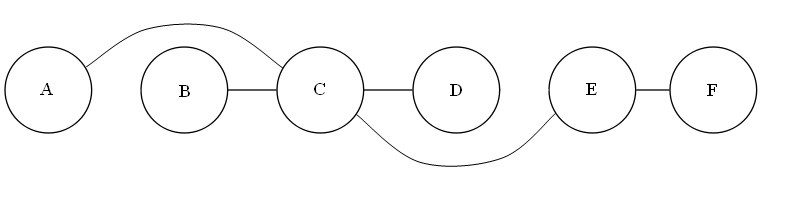
\includegraphics[scale=.4]{figures/tree.png}
&
\begin{tabular}{c|c|c}
\AnswerOneBi
\end{tabular}
\end{tabular}
\end{table}\\

\end{subquestion}
\begin{subquestion}[6]{}\\
For each algorithm, circle all orderings of variable assignments that guarantee that no more than two variables will be backtracked when finding a solution to the CSP represented by the following constraint graph.\\\\

\begin{table}[h]
\centering
\begin{tabular}{cc}
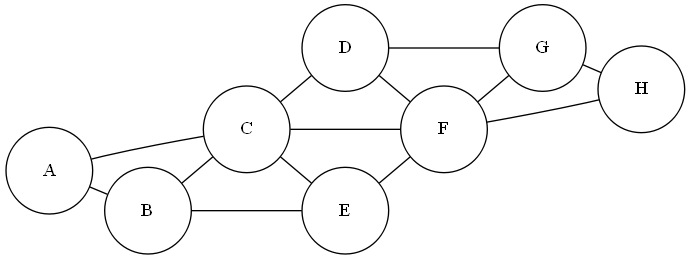
\includegraphics[scale=.3]{figures/csp_graph.png}
&
\begin{tabular}{c|c|c}
\AnswerOneBii
\end{tabular}
\end{tabular}
\end{table}
\end{subquestion}
\end{question}
\newpage
\begin{question}[]{\bf All Satisfying Assignments}
Now consider a modified CSP in which we wish to find every possible satisfying assignment, rather than just one such assignment as in normal CSPs. In order to solve this new problem, consider a new algorithm which is the same as the normal backtracking search algorithm, except that when it sees a solution, instead of returning it, the solution gets added to a list, and the algorithm backtracks. Once there are no variables remaining to backtrack on, the algorithm returns the list of solutions it has found.\\\\
For each graph below, select whether or not using the MRV and/or LCV heuristics could affect the number of leaf nodes in the search tree in this new situation.


\begin{subquestion}[2]{}\\
\begin{tabular}{cl}
\multirow{1}{*}{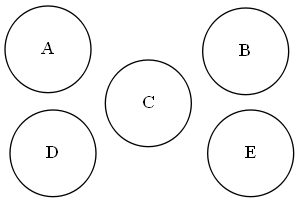
\includegraphics[scale=0.5]{figures/disconnected.png} \hspace{1.4in}}
\AnswerOneCi

\end{tabular}\\
\end{subquestion}

\vspace{-.1in}
\begin{subquestion}[2]{}\\
\begin{tabular}{cl}


\multirow{1}{*}{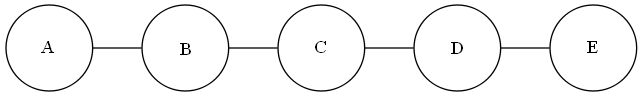
\includegraphics[scale=0.5]{figures/chain.png} \hspace{0.260in}}
\AnswerOneCii

\end{tabular}\\
\end{subquestion}
\vspace{-.19in}
\begin{subquestion}[2]{}\\
\begin{tabular}{cl}

\multirow{1}{*}{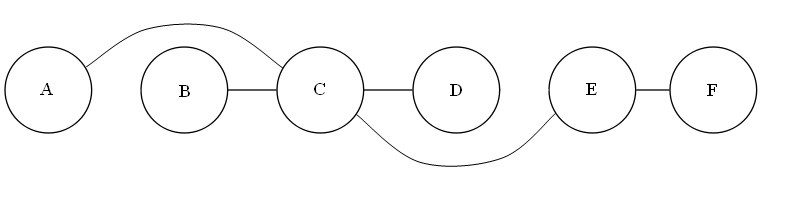
\includegraphics[width=3in]{figures/tree.png}}\\\\
\AnswerOneCiii

\end{tabular}
\end{subquestion}
\vspace{-.19in}
\begin{subquestion}[2]{}\\
\begin{tabular}{cl}

\multirow{1}{*}{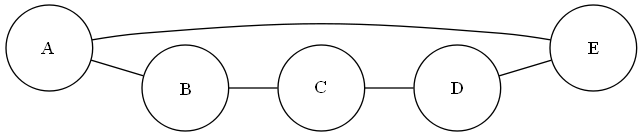
\includegraphics[width=3in]{figures/circle.png}} \\\\
\AnswerOneCiv

\end{tabular}
\end{subquestion}

\vspace{-.15in} 
\begin{subquestion}[2]{}\\
\begin{tabular}{cl}

\multirow{1}{*}{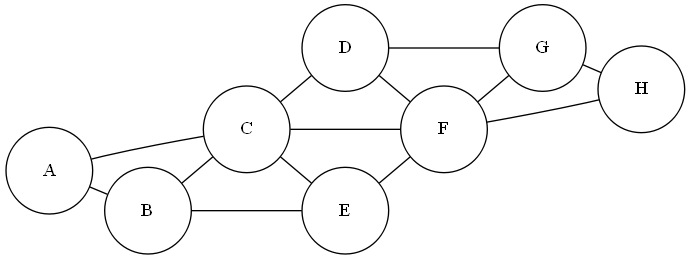
\includegraphics[width=3in]{figures/csp_graph.png}} \\\\
\AnswerOneCv

\end{tabular}
\end{subquestion}



\end{question}
\newpage
\begin{problem}[]{Preprocessing Bayes' Net Graphs for Inference}

\begin{tabular}{ll}
\begin{minipage}{0.7\textwidth}
For (a) and (b), consider the Bayes' net shown on the right.  You are given
the structure but you are not given the
conditional probability tables (CPTs).  We will consider the query $P(B|+d)$,
and reason about which steps in the variable elimination process we might be able
to execute based on just knowing the graph structure and not the CPTs.
\end{minipage}
&
\begin{minipage}{0.25\textwidth}
\begin{figure}[H]
\centering
    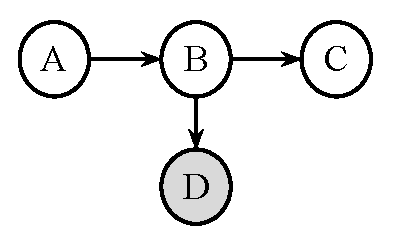
\includegraphics[width=0.8\textwidth]{figures/FA12-MT2-Elimination3V1.pdf}
\end{figure}
\end{minipage}
\\
\end{tabular}
\begin{question}[2]
Assume the first variable we want to eliminate is $A$ and the
resulting factor would be $f_1(B)$. Mark which one of the following is true.
\begin{multicols}{3}
\begin{itemize}[label=, itemsep=12pt, topsep=12pt]
\TwoA
\end{itemize}
\end{multicols}
\solution{\vspace{0.5in}}{
   \fbox{\begin{minipage}[t][2.0cm][t]{18cm} 2a Explanation: \TwoAExplanation \end{minipage}}\\
}
\end{question}

\begin{question}[2]
Assume the first variable we eliminate is $C$ and the resulting factor is $g_1(B)$. Mark which one of the following is true.
\begin{multicols}{3}
\begin{itemize}[label=, itemsep=12pt, topsep=12pt]
\TwoB
\end{itemize}
\end{multicols}
\solution{\vspace{0.5in}}{
   \fbox{\begin{minipage}[t][2.0cm][t]{18cm} 2b Explanation: \TwoBExplanation \end{minipage}}\\
}
\end{question}

\begin{tabular}{ll}
\begin{minipage}{0.7\textwidth}
For (c) through (g),  consider the Bayes' net shown on the right.  You are given
the structure but you are not given the
conditional probability tables (CPTs).  We will consider the query $P(B|+g)$,
and again we will reason about which steps in the variable elimination process we might be able
to execute based on just knowing the graph structure and not the CPTs.
\end{minipage}
&
\begin{minipage}{0.25\textwidth}
\begin{figure}[H]
\centering
    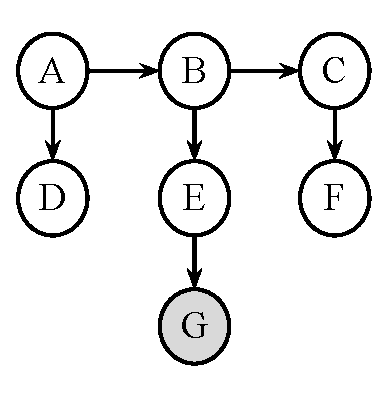
\includegraphics[width=0.6\textwidth]{figures/FA12-MT2-Elimination3V2.pdf}
\end{figure}
\end{minipage}
\\
\end{tabular}


\begin{question}[2]
Assume the first variable we eliminate is $D$ and the resulting factor is $h_1(A)$. Mark which one of the following is true.
\begin{multicols}{3}
\begin{itemize}[label=, itemsep=12pt, topsep=12pt]
\TwoC
\end{itemize}
\end{multicols}
\solution{\vspace{0.5in}}{
   \fbox{\begin{minipage}[t][2.0cm][t]{18cm} 2c Explanation: \TwoCExplanation \end{minipage}}\\
}
\end{question}

\begin{question}[2]
Assume the first 2 variables we eliminate are $A$ and $D$ and the resulting factor is $i_2(B)$. Mark which one of the following is true.
\begin{multicols}{3}
\begin{itemize}[label=, itemsep=12pt, topsep=12pt]
\TwoD
\end{itemize}
\end{multicols}
\solution{\vspace{0.5in}}{
   \fbox{\begin{minipage}[t][2.0cm][t]{18cm} 2d Explanation: \TwoDExplanation \end{minipage}}\\
}
\end{question}

\begin{question}[2]
Assume the first variable we eliminate is $F$ and the resulting factor is $j_1(C)$. Mark which one of the following is true.
\begin{multicols}{3}
\begin{itemize}[label=, itemsep=12pt, topsep=12pt]
\TwoE
\end{itemize}
\end{multicols}
\solution{\vspace{0.5in}}{
   \fbox{\begin{minipage}[t][2.0cm][t]{18cm} 2e Explanation: \TwoEExplanation \end{minipage}}\\
}
\end{question}

\begin{figure}[H]
\centering
    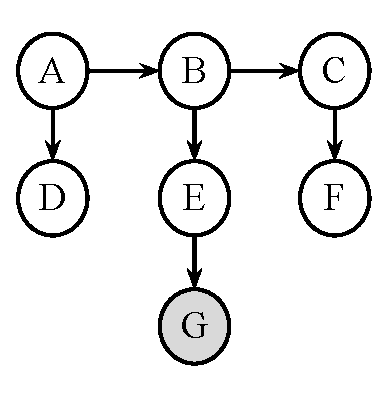
\includegraphics[width=0.15\textwidth]{figures/FA12-MT2-Elimination3V2.pdf}
\caption*{For your convenience we included the Bayes' Net structure
  again on this page.}
\end{figure}
\vspace{-0.2in}

\begin{question}[2]
Assume the first 2 variables we eliminate are $F$and $C$ and the resulting factor is $k_2(B)$. Mark which one of the following is true.
\begin{multicols}{3}
\begin{itemize}[label=, itemsep=12pt, topsep=12pt]
\TwoF
\end{itemize}
\end{multicols}
\solution{\vspace{0.5in}}{
   \fbox{\begin{minipage}[t][2.0cm][t]{18cm} 2f Explanation: \TwoFExplanation \end{minipage}}\\
}
\end{question}

\begin{question}[2]
Assume the first variable we eliminate is $E$ and the resulting factor is $l_1(B,+g)$. Mark which one of the following is true.
\begin{multicols}{3}
\begin{itemize}[label=, itemsep=12pt, topsep=12pt]
\TwoG
\end{itemize}
\end{multicols}
\solution{\vspace{0.5in}}{
   \fbox{\begin{minipage}[t][2.0cm][t]{18cm} 2g Explanation: \TwoGExplanation \end{minipage}}\\
}
\end{question}


\begin{question}[4]
In the smaller examples in (a) through (g) you will have observed that
sometimes a variable can be eliminated without knowing any of the CPTs.
This means that variable's CPT does not affect the answer to the
probabilistic inference query and that variable can be removed from the graph for
the purposes of that probabilistic inference query.  Now consider the following,
larger Bayes' net with the query $P(Q|+e)$.\\


\begin{figure}[4]
\centering
    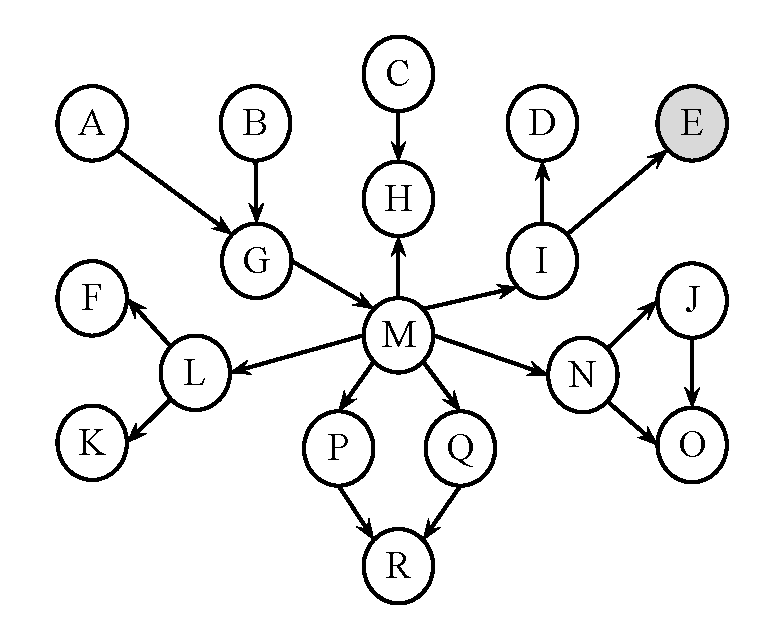
\includegraphics[width=0.5\textwidth]{figures/FA12-MT2-Elimination3V3.pdf}
\end{figure}
Mark all of the variables whose CPTs do \textit{not} affect the value of $P(Q|+e)$:

\begin{center}
\begin{tabular}{lllll}
\TwoH
\end{tabular}
\end{center}
\solution{\vspace{0.5in}}{
   \fbox{\begin{minipage}[t][2.0cm][t]{18cm} 2h Explanation: \TwoHExplanation \end{minipage}}\\
}
\end{question}
\end{problem}
\newpage


\end{document}